\chapter{Certification}
\label{chap_certification}

\targets{
  \item Know important domains of safety-critical software systems.
  \item Understand that domains have different requirements, regulation and certification standards.
  \item Understand differences in certification processes.
}




\begin{frame}{Certification Standards}
	Domain-specific certification standards:
	
	\begin{beameritemize}
		\item Medical devices: IEC 62304, IEC 82304 (Complies with Medizinproduktegesetz)
		\item Avionic: DO-178C
		\item Automotive: ISO 26262 
	\end{beameritemize}
\end{frame}


\section{Medical Devices}

\begin{frame}{Medical Devices Directive (in the EEA)}
	Medical Devices Directive:
	\begin{beameritemize}
		\item Introduced with the intention to harmonize medical devices laws in the European Economic Area (EEA).
		\item Members of the EEA have to adjust their national laws and regulations according to the MDD in order to create common standards across the EEA.\\
		$\Rightarrow$ If a medical device is approved in one country, it can be exported to other country inside the EEA.
		\item CE marking shows that the product meets standards.
	\end{beameritemize}	

  	\xxx
	\centering
	
\includegraphics[width=0.1\linewidth]{content/images/certification/CE}
\end{frame}



\begin{frame}{Medizinproduktegesetz (in Germany)}
	\begin{beameritemize}
		\item German law that is conform with the Medical Devices Directive.
		\item High individual responsibility of the manufacturers. 
		\item Categorized in risk classes on which the certification is depending on.
	\end{beameritemize}	
\end{frame}

\begin{frame}{Medizinproduktegesetz (in Germany)}
	Categorized in risk classes:	
	\begin{block}{Class I}
		\begin{columns}[c]
			\column{2in}
			\begin{beameritemize}
				\item low risk
				\item non-invasive
				\item reusable
			\end{beameritemize}			
			\column{2in}
			Examples:\\
			Glasses, wheelchairs, bandages
		\end{columns}		
	\end{block}
	
	\begin{block}{Class IIa}
		\begin{columns}[c]
			\column{2in}
			\begin{beameritemize}
			\item medium risk
			\item invasive or non-invasive over a short period of time
		\end{beameritemize}		
			\column{2in}
			Examples:\\
			Syringes, ultrasound, MRI
		\end{columns}		
	\end{block}
\end{frame}


\begin{frame}{Medizinproduktegesetz (in Germany)}
	Categorized in risk classes:	
	\begin{block}{Class IIb}
		\begin{columns}[c]
			\column{2in}
			\begin{beameritemize}
				\item increased risk
				\item implantable or invasive for a long period of time
			\end{beameritemize}	
			\column{2in}
			Examples:\\
			Medical ventilator, defibrillator
		\end{columns}		
	\end{block}
	
	\begin{block}{Class III}
		\begin{columns}[c]
			\column{2in}
			\begin{beameritemize}
				\item high risk
				\item highly (or surgically) invasive over a long period of time
			\end{beameritemize}
			\column{2in}
			Examples:\\
			Cardiac catheters, stents, implants
		\end{columns}	
	
	\end{block}
\end{frame}



\begin{frame}{Medizinproduktegesetz (in Germany)}
	\begin{beameritemize}
		\item Conformity assessment procedures (German: "Konformitätsbewertungsverfahren") have to be performed.
		\item Manufacturer must provide documented proof of conformity with regulatory requirements.
		\item Risk classes II and III are controlled by a "Notified Body" (German:"Benannte Stelle")
	\end{beameritemize}
\end{frame}


\begin{frame}{Medizinproduktegesetz (in Germany)}
	Software:
	\begin{beameritemize}
		\item as part of a medical device (software is certified during the regular process)
		\item as standalone medical device ($\Rightarrow$ IEC 62304)
		\item as a component for another medical device ($\Rightarrow$ IEC 62304)
	\end{beameritemize}
	\xxx
	$\Rightarrow$ IEC 62304 only requires quality and risk management. No explicit verification techniques are specified.

\end{frame}

\begin{frame}{Medizinproduktegesetz (in Germany)}
	\begin{block}{Standalone Medical Software}
		Standalone software is a medical device if the intended purpose of the manufacturer corresponds to the definition of a medical device. 
	\end{block}
		
	For example: Picture archiving and Communication System.
	
	\centering
	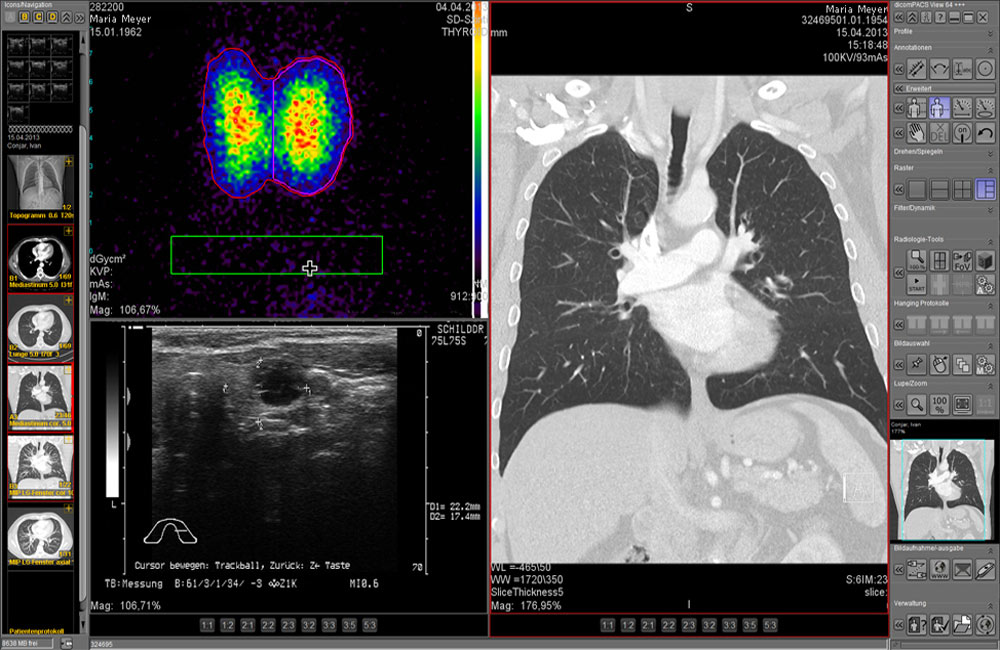
\includegraphics[width=0.7\linewidth]{content/images/certification/PACS}

	

\end{frame}


\begin{frame}{Medizinproduktegesetz (in Germany)}

	\begin{block}{Modular Medical Devices}
		If the software consists of multiple modules, only those have to fulfill requirements of medical devices which have a medical intended purpose.
	\end{block}
	\xxx
	For example: A hospital IT-system that consists of a financial part and a medication/prescription part. Only the later module has to comply  with the laws of medical devices.
\end{frame}



\begin{frame}{Harmonized Norms}
	Based on the laws there are harmonized norms, that can be used by manufacturer to get the development process approved:
	\xxx
	\begin{beameritemize}
		\item ISO 13485 (Quality Management)
		\item ISO 14971 (Risk Management)
		\item ISO 62366 (Usability of Medical Devices)
		\item IEC 62304 (Software of Medical Devices)
		\item ...
	\end{beameritemize}	
	
\end{frame}

\begin{frame}{Quality Management (ISO 13485)}
	\begin{beameritemize}
		\item Documentation of processes and development phases in the company
		\item From first product planning to market observation\\
		 $\Rightarrow$ QM-documents, source code, logs, test protocols...
		\item Additionally, assurance of quality of bought-in parts
	\end{beameritemize}	
	
	
\end{frame}


\begin{frame}{Risk Management (ISO 14971)}
	\begin{beameritemize}
		\item For each part of the product has to be assessed how it could fail and what its risk potential is.
		\item The risk potential depends on the likelihood of the failure and the severity of it.		 
	\end{beameritemize}	
	\xxx
	\centering
	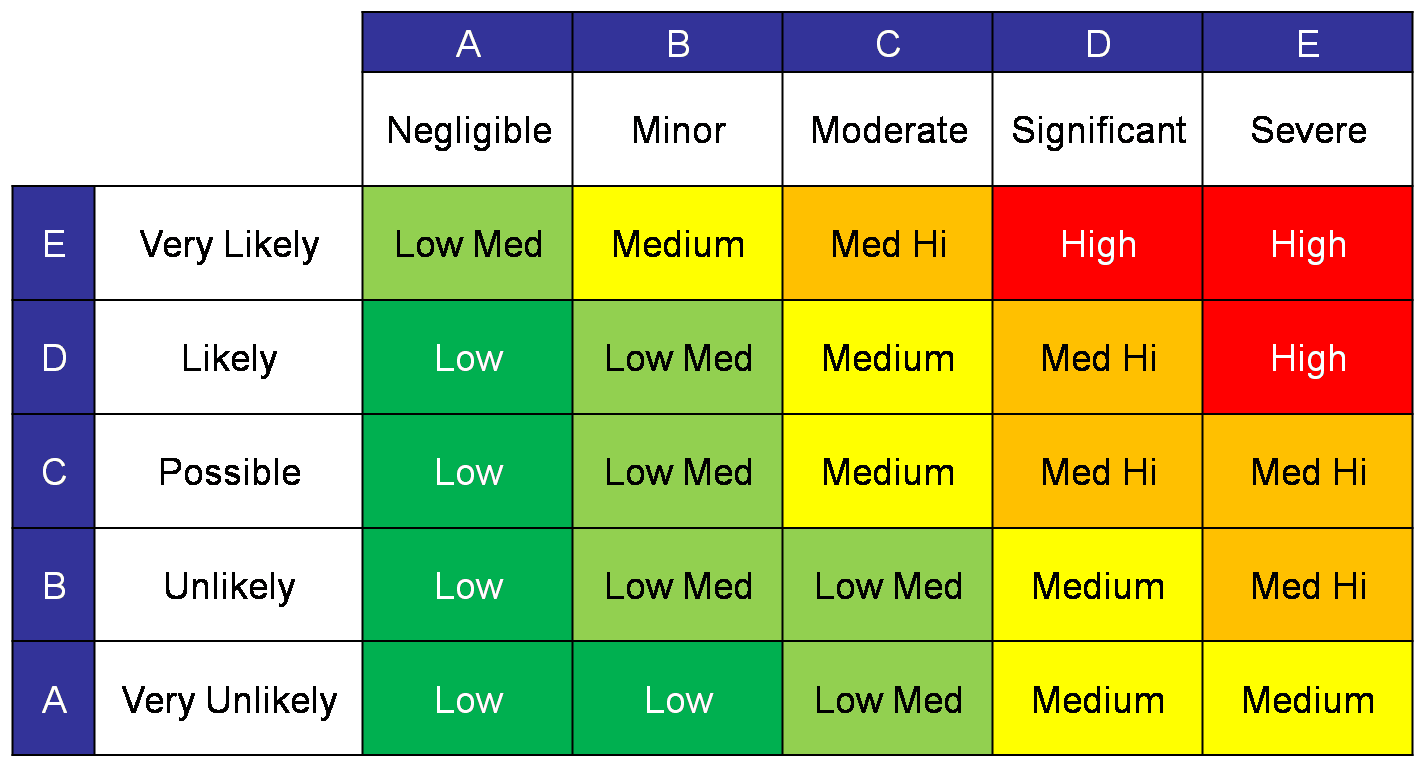
\includegraphics[width=0.7\linewidth]{content/images/certification/risk_matrix}
\end{frame}


\begin{frame}{Risk Management (ISO 14971)}
	Methods:
	\begin{beameritemize}
		\item Preliminary Hazard Analysis (PHA)
		\item Fault Tree Analysis (FTA)
		\item Failure Mode and Effects Analysis (FMEA) 
		\item Hazard and Operability Study (HAZOP)
	\end{beameritemize}	
	\xxx
	$\Rightarrow$ Next week: More about risk management and FMEA by Plato!
	
	
\end{frame}


\section{Automotive}

\begin{frame}{ISO 26262}	
	\begin{block}{ISO 26262}
	is the international standard in the domain of automotive for electrical and electronic components.
	\end{block}
	\xxx
	Goals:
	\begin{beameritemize}
		\item Providing functional safety of electrical systems.
		\item Covering safety aspects of the whole software life cycle but especially during the development process.
		\item Automotive-specific risk assessment and management including safety levels (ASILs).
	\end{beameritemize}
\end{frame}


\begin{frame}{ISO 26262 - Software}	
	Requirements on software are defined in ISO 26262:
	
	\begin{beameritemize}
		\item V-model has to be used throughout the development process.
		\item ASIL level defines which requirements are highly recommended and which are optional.
		\item Requirements have to be traceable.
		\item Guidelines are used for software development, typically MISRA C.
		\item Verification focuses mostly on testing.
	\end{beameritemize}

\begin{center}
	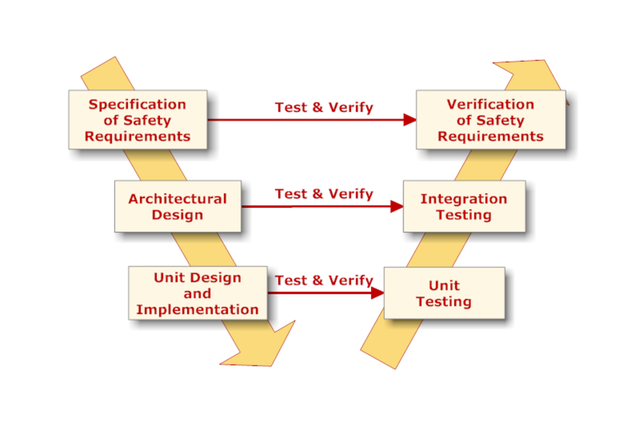
\includegraphics[width=0.7\linewidth]{content/images/certification/iso26262vmodel}
\end{center}

\end{frame}

\begin{frame}{ISO 26262}
	\begin{beameritemize}
		\item As the complexity of a system increases, the risk of systematic failures and random hardware failures increases.
	\end{beameritemize}	

	\begin{block}{Functional Safety}
		is the absence of unreasonable risk due to hazards caused by malfunctioning behavior of electrical and electronic systems.
	\end{block}	
\end{frame}


\begin{frame}{ISO 26262}	
	Functional safety is classified as Automotive Safety Integrity Levels (ASIL A-D) by evaluating three factors severity, exposure and controllability :\\
	\xxx
	
	\begin{zebratabular}{ll}
		\headerrow Severity & Consequences of a failure: \\
		S0 & No injuries\\
		S1 & Minor or medium injuries\\
		S2 & Major injuries, but probably no fatalities\\
		S3 & Major injuries and fatalities
	\end{zebratabular}

	
\end{frame}


\begin{frame}{ISO 26262}	
	
	\begin{zebratabular}{ll}
		\headerrow Exposure & Probability of a failure: \\
		E0 & Rare\\
		E1 & Occasional\\
		E2 & Frequently\\
		E3 & Constant
	\end{zebratabular}

	\xxx

	\begin{zebratabular}{ll}
		\headerrow Controllability & Correction of a failure by the driver: \\
		C0 & Safe\\
		C1 & Easy\\
		C2 & Normal\\
		C3 & Hard
	\end{zebratabular}

\end{frame}

\begin{frame}{ISO 26262}	
	Based on these factor (S, E, C) the classification can be determined using the ASIL-table (QM means that regular quality management is sufficient):
	
	\centering
	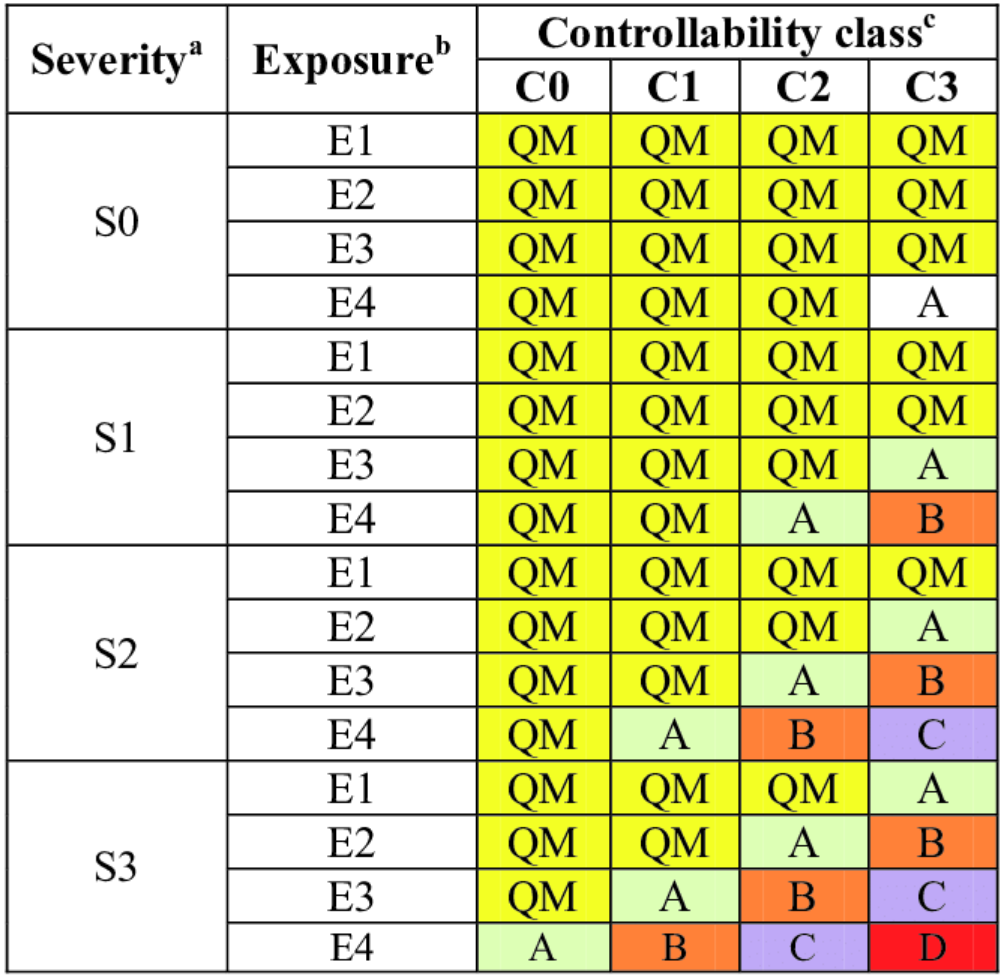
\includegraphics[width=0.7\linewidth]{content/images/certification/asil-table}

\end{frame}

\begin{frame}{ISO 26262}	
	Examples:\\
	\xxx
	
	\begin{zebratabular}{ll}
		\headerrow ASIL & Functionality: \\
		A & Window lifter \\
		B & Break light\\
		C & ESP\\
		D & Electrical steering wheel lock
	\end{zebratabular}
	
	
\end{frame}






\begin{frame}{ISO 26262 - Software}		
	Example: Methods for software unit testing (ISO 26262 Table 10)\\
	\xxx
	\begin{zebratabular}{lllll}
		\headerrow Method  & A & B & C & D \\
		Requirement-based testing & ++ & ++ & ++ & ++ \\
		Interface test & ++ & ++ & ++ & ++\\
		Fault injection test & + & + & + & ++ \\
		Resource usage test & + & + & + &  ++ \\
	\end{zebratabular}

	++: highly recommended\\
	+: recommended 
	
\end{frame}


\begin{frame}{ISO 26262 - Software}		
	Example: Methods for deriving testcases for integration testing (part of ISO 26262-4 Table 4)\\
	\xxx
	\begin{zebratabular}{lllll}
		\headerrow Method  & A & B & C & D \\
		Analysis of requirements & ++ & ++ & ++ & ++ \\
		Analysis of boundary values & + & + & ++ & ++ \\
		Error guessing based on knowledge & + & + & ++ &  ++ \\
		Analysis of functional dependencies & + & + & ++ &  ++ \\
	\end{zebratabular}

	++: highly recommended\\
	+: recommended 
	
\end{frame}

\begin{frame}{ISO 26262 - Software}		
	Example: Code Coverage Requirements (part of ISO 26262-4 Table 6)\\
	\xxx
	\begin{zebratabular}{lllll}
		\headerrow Coverage  & A & B & C & D \\
		MC/DC & + & + & + & ++ \\
		Decision & + & ++ & ++ & ++ \\
		Statement & ++ & ++ & + &  + \\
	\end{zebratabular}
	
	++: highly recommended\\
	+: recommended 
	
\end{frame}




\section{Avionics}

\begin{frame}{DO-178C}
	
	\begin{block}{Definition}
	DO-178C, Software Considerations in Airborne Systems and Equipment Certification, is used to approve commercial software-based aerospace systems by certification authorities.
	\end{block}
	\xxx
	
	\begin{beameritemize}
		\item Regulated by the FAA (Federal Aviation Administration)
		\item Applies only to software, not hardware
		\item Covers the full engineering life cycle (planning, development, verification)
		\item The Design Assurance Level (DAL) of a system is determined by examining the effects of a failure in the system.
		\item Depending on the DAL, different objectives need to be fulfilled during the development phase.
	\end{beameritemize}
		
\end{frame}


\begin{frame}{DO-178C}
	Design Assurance Level (DAL):\\
	\xxx
	
	\begin{zebratabular}{llll}
		\headerrow Effect:  & ~ & DAL: & \#Obj. \\
		Catastrophic  & (multiple fatalities) & A & 71\\
		Hazardous & (serious or fatal injuries) & B & 69 \\
		Major & (discomfort or minor injuries) & C & 62 \\
		Minor & (inconvenience) & D & 26 \\
		No Effect & ~ & E & 0*\\
	\end{zebratabular}
	\xxx
	* Just prove you are level E.
	
\end{frame}

\begin{frame}{DO-178C}
	
	Easy to confuse:
	\xxx
	\begin{center}
		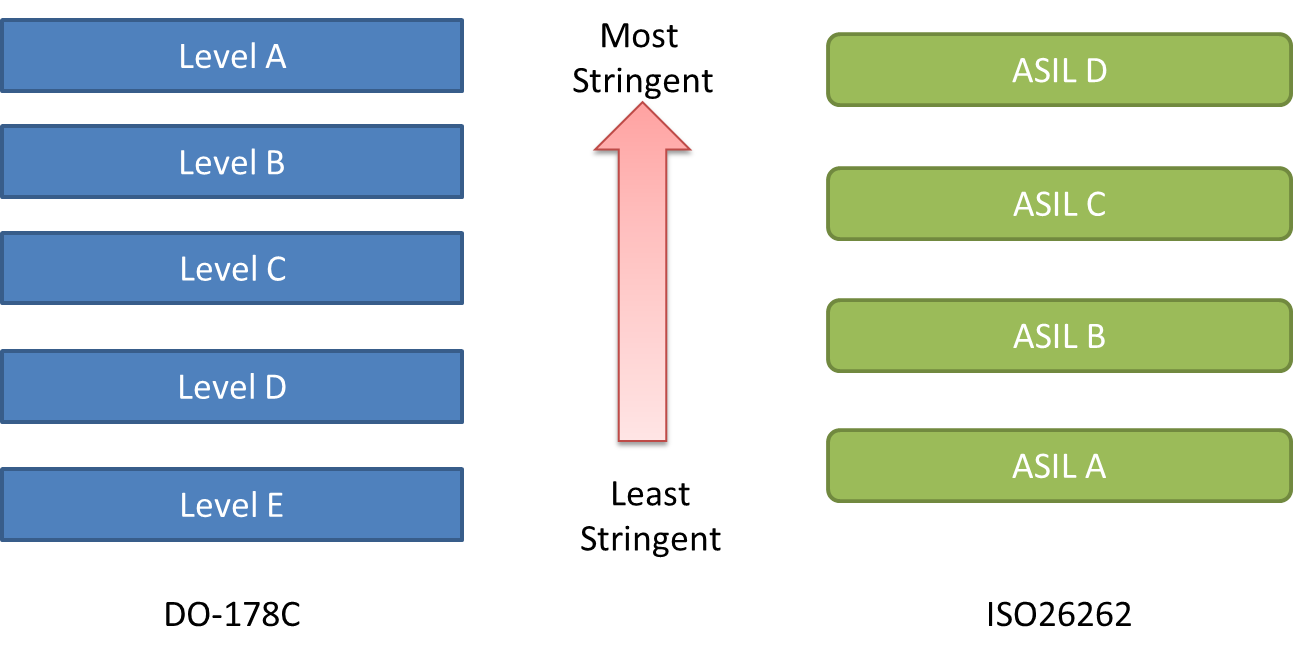
\includegraphics[width=0.9\linewidth]{content/images/certification/DALvsASIL}
	\end{center}
\end{frame}

\begin{frame}{DO-178C}
	Key attributes:
	\begin{beameritemize}
		\item Detailed planning
		\item Criticality Levels (DAL A-E)
		\item Consistency
		\item Traceability
		\item Independence
		\item Path testing
		\item Use of qualified tools
		\item ''Guilty until proven innocent''
	\end{beameritemize}
	
\end{frame}

\begin{frame}{DO-178C}
	Key plans (all DALs):
	\begin{beameritemize}
		\item PSAC: Plan for SW aspects of certification
		\item SQAP: SW quality assurance plan
		\item SCMP: SW configuration management plan
		\item SWDP: SW development plan
		\item SWVP: SW verification plan
	\end{beameritemize}
	\xxx
	For DAL A,B,C applicants also have to develop:\\
	\begin{beameritemize}
		\item SCS: SW coding standard
		\item SRS: SW requirements standard
		\item SDS: SW design standard
	\end{beameritemize}
		
\end{frame}




\begin{frame}{DO-178C}
	Structural code coverage:
	\xxx
	\begin{zebratabular}{llllll}
		\headerrow Coverage  & A & B & C & D & E \\
		MC/DC & yes & - & - & - & - \\
		Decision & yes & yes & - & - & -\\
		Statement & yes & yes & yes & - & - \\
	\end{zebratabular}

	\xxx
	Note: For level A and B the testing process has to be performed by someone not directly involved with the development process.
\end{frame}


\begin{frame}{DO-178C}
Other objectives:
\xxx
\begin{zebratabular}{llllll}
	\headerrow Objective:  & A & B & C & D & E \\
	Source to Binary correlation & yes & - & - & - & - \\
	Code reviews & yes & yes & - & - & -\\
	Low-level requirements & yes & yes & yes & - & - \\
\end{zebratabular}


\end{frame}

\begin{frame}{DO-178C}
	Traceability:\\
	\xxx
	\centering
	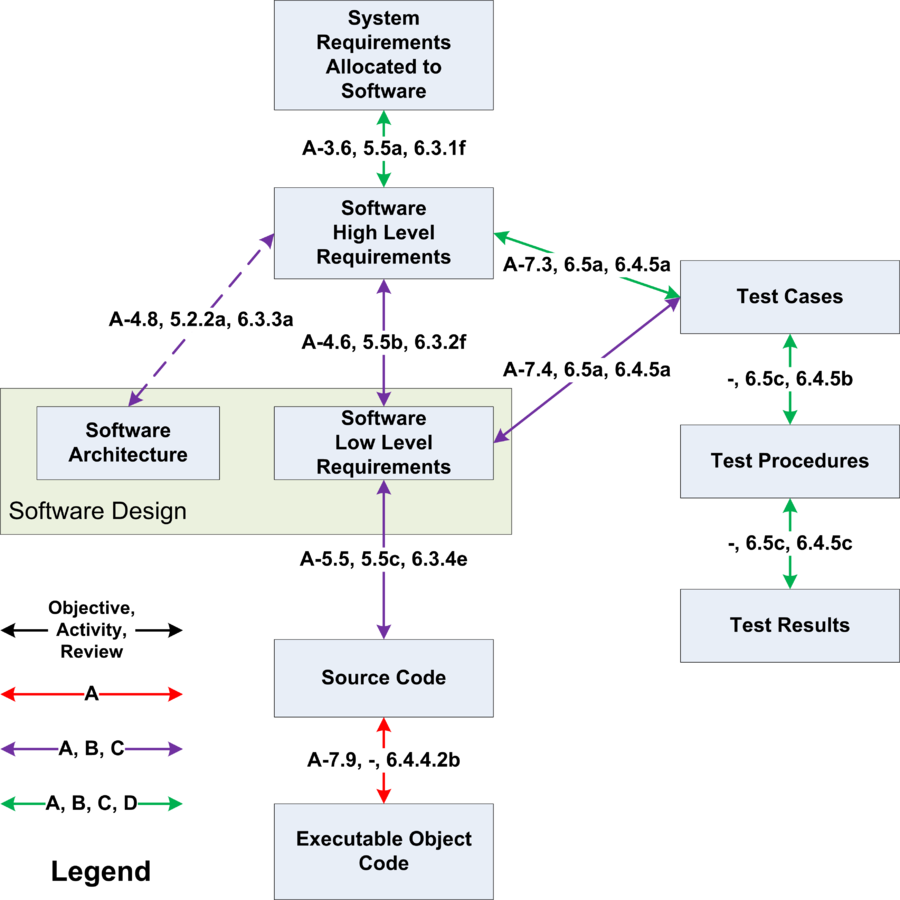
\includegraphics[width=0.8\linewidth]{content/images/certification/traceability}
\end{frame}


\begin{frame}{DO-178C}
	Developing SW for aircrafts (estimation for level B):
	\begin{beameritemize}
		\item Quality Assessment: 10 \%
		\item Management: 10 \%
		\item Requirements Development: 10 \%
		\item Code Design: 10 \%
		\item Actual Coding: 25 \%
		\item Verification: 35 \%
	\end{beameritemize}
	\xxx
	$\Rightarrow$ Very costly\\
	\xxx	
	$\Rightarrow$ More time is spend for verification than for coding.
\end{frame}


\subsection*{Conclusion}

\begin{frame}{Conclusion}
	\begin{enumerate}
		\item Certification processes assure a certain degree \alert{functional safety}.
		\item Depending on the severity of failure different \alert{software level} are defined (DAL, ASIL).
		\item Depending on the software levels and the domain different \alert{objectives} must be fulfilled during software development.
	\end{enumerate}
\end{frame}




\mode
<all>